\section{Flusso di progetto nei sistemi eterogenei}\label{capitolo3}
Come abbiamo visto i sistemi embedded sono sistemi specializzati progettati per svolgere una o poche funzioni, molto spesso con vincoli stringenti. Questi tipi di sistemi sono progettati come \emph{SoC Multiprocessore} che sono diventati lo  standard di fatto di questo tipo di sistemi. Molti dei sistemi embedded hanno dei vincoli stringenti per quanto riguarda le prestazioni, l'ottimizzazione delle applicazioni per sistemi embedded complessi è un problema difficile, che richiede progettisti con un alto livello di esperienza per identificare la soluzione migliore.\\
Solitamente si utilizzano delle piattaforme hardware di base, tuttavia i vincoli stringenti richiedono processori dedicati per accelerare specifiche funzioni.\\
Per definire il problema dobbiamo considerare numerosi aspetti:
\begin{description}
\item[Job:] ovvero l'attività da eseguire e completare affinché il sistema soddisfi le specifiche.
\item[Punto di implementazione:] indica il modo nel quale svolgere un lavoro. Rappresenta una combinazione di \emph{latenza} e \emph{risorse necessarie}.
\item[Mapping:] assegna ogni \emph{job} ad un possibile \emph{punto di implementazione}, in modo da rispettare i vincoli imposti dalle risorse.
\item[Scheduling:] determina l'ordine di esecuzione di tutti i lavori.
\item[Obiettivo:] minimizzare il tempo di esecuzione complessivo dell'applicazione sull'architettura designata
\end{description}
Per quanto riguarda l'\emph{obiettivo} di minimizzare il tempo di esecuzione possiamo intervenire in diversi modi, come quello di analizzare, valutare ed ottimizzare differenti alternative, ed una volta individuata una soluzione valutarne la qualità prima della sua implementazione.\\
La progettazione di sistemi eterogenei a multi processore richiede diversi fasi:
\begin{itemize}
\item Una fase di partizionamento dell'applicazione (\emph{partitionig})
\item Una fase di assegnamento dei task ai diversi elementi architetturali (\emph{mapping})
\item La determinazione dell'ordine di esecuzione dei task (\emph{scheduling})
\end{itemize}
La parte di \emph{scheduling} e di \emph{mapping} è un problema \emph{NP-completo} inoltre il problema di un design e l'interfacciamento di componenti eterogenei può generare delle soluzioni non ammissibili.\\
Una rappresentazione imparziale e unificata di software ed hardware supporta la fase di progettazione ed analisi, permette una facile valutazione delle soluzioni individuate e inoltre permette la migrazione dei task tra la parte hardware e quella software. Tecniche di progettazione iterative permettono di valutare soluzioni differenti, aiuta a determinare l'implementazione migliore ed infine il partizionamento dei moduli permette un maching più preciso rispetto ai criteri di progettazione. Esistono inoltre dei metodi di parallelizzazione che possono valutare il grado di parallelismo a livello di :
\begin{itemize}
\item Istruzione
\item Dati 
\item Task
\end{itemize}
Tuttavia si introducono problemi di dipendenza che devono essere soddisfatti.\\
il parallelismo dei dati è definito come il parallelismo ottenuto dall'esecuzione concorrente che utilizza porzioni di dati differenti.
Il parallelismo dei task invece viene definito come il parallelismo ottenuto dalla computazione su diverse strutture dati.
In molti casi si utilizza un misto delle due tecniche soprattutto in ambito scientifico.\\
Un \emph{grafico dei task} è un grafico $G=(T,E)$ nei quali i nodi rappresentano un gruppo di istruzioni e gli archi rappresentano le dipendenze, solitamente gli archi vengono indicati con il quantitativo di dati da trasferire in modo da considerare anche il ritardo di comunicazione.
Nel caso di grafi ciclici adotteremo la rappresentazione \emph{gerarchica dei grafi} nei quali i nodi son suddivisi in tre classi:
\begin{description}
\item[semplici:] un task senza altri sotto task,
\item[composto:] quando un task ha altri sotto task associati,
\item[loop:] task che rappresentano un ciclo in cui il corpo è un sotto-grafo
\end{description}
I meccanismi utilizzati per l'analisi devo preservare il \emph{comportamento osservabile} del programma, ovvero, consumare i bytes in input, rispettare l'output e la terminazione del programma; tuttavia l'output può subire alcune variazioni come una differente precisione o operazioni associate in modo diverso ma il compilatore deve dimostrare che le trasformazioni preservano il comportamento in caso contrario le ottimizzazioni devono essere conservative.\\
\subsection{Analisi delle dipendenze}
Un linguaggio sequenziale presenta un ordinamento totale dei vari blocchi, tuttavia per mantenere il comportamento osservabile del programma è sufficiente un \emph{ordinamento parziale} ma questo ordinamento deve essere scoperto. Prendiamo come esempio il codice seguente:
\begin{verbatim}
float foo(a, b) {
    float t1 = sin (a);
    float t2 = cos (b);
    return t1/t2;
}
\end{verbatim}
In questo caso riordinando \emph{t1} e \emph{t2} il comportamento della funzione non cambia. L'ordinamento nel codice sorgente risulta essere pessimistico, un analisi delle dipendenze individua in modo più specifico un ordinamento parziale e questo da la libertà al compilatore di risistemare il codice. L'analisi però risulta in molti casi \emph{incompleta}, infatti, nel caso migliore risulta \emph{precisa} in quello peggiore, invece, tende ad essere molto \emph{conservativa} questo porta alla creazione di false dipendenze che possono essere rimosse soltanto migliorando l'analisi.\\
Vediamo ora quali sono le tipologie di dipendenza analizzando come prima la dipendenza dei dati, il codice di esempio mostra un tipico caso di dipendenza dei dati dove un'operazione utilizza il valore proveniente da un'operazione precedente, si può costruire anche un grafico delle dipendenze come quello in \figurename\,\ref{fig:datadep}.
\begin{verbatim}
P = ...;
Q = ...;
R = P + Q;
S = Q + 1;
\end{verbatim}
\begin{figure}
\centering
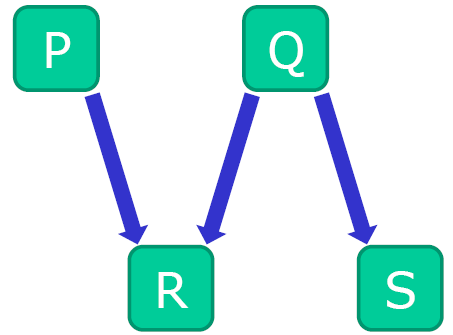
\includegraphics[scale=0.5]{img/datadep.png}
\caption{Esempio di grafico delle dipendenze sui dati}\label{fig:datadep}
\end{figure}
Esistono diverse categorie di dipendenze dei dati:
\begin{itemize}
\item Dipendenza \emph{flow} o anche \emph{Read After Write}
\item Dipendenza \emph{anti} o anche \emph{Write After Read}
\item Dipendenza \emph{output} o anche \emph{Write After Write}
\end{itemize}
Tuttavia le ultime due dipendenze sono tali a causa di riuso delle risorse e non sono vere dipendenze dei dati.\\
La seconda dipendenza che analiziamo è la \emph{dipendenza da controllo} in questo caso la dipendenza è dovuta al fatto che un'operazione può essere abilitata o disabilitata dall'esecuzione di un'altra istruzione come avviene nel caso di un costrutto \texttt{if}. In alcuni casi è possibile rimuovere alcune dipendenze come nell'esempio seguente:
\begin{verbatim}
if (P) {
    X = Y + 1;
    print(X);
}
\end{verbatim}
In questo caso è possibile eseguire l'istruzione che assegna il valore \emph{X} al di fuori dell'istruzione di controllo senza modificare il comportamento del programma.\\
L'analisi delle dipendenze tuttavia no è banale, un metodo come detto è quello che utilizza grafi delle dipendenze ma risulta di difficile computazione ed inoltre alcuni loop non sono esplicitati questo potrebbe portare a dipendenze non risolte. Un'altra metodologia è quella del \emph{task partitioning} nel quale di divide il problema assegnato in sottoproblemi come segue:
\begin{description}
\item[Obiettivi:] l'obiettivo primario viene suddiviso in \emph{n} sotto obbiettivi $O=\{o_1,o_2,\dots, o_n\}$ composti da 
\item[Blocchi:] o anche chiamati \emph{partizioni} $P=\{p_1,\dots, p_m$
\end{description}
queste partizioni devo rispettare alcune proprietà:
\begin{itemize}
\item $p_1 \cup p_2 \cup \dots \cup p_m = O$
\item $p_i\cap p_j = \emptyset \forall i\neq j$
\item la funzione di costo $c(P)$ deve essere minimizzata.
\end{itemize}
Tale funzione di costo esprime la qualità del sistema e può includere il \emph{costo del sistema}, la \emph{latenza} e il \emph{consumo di energia}.
Esistono diversi metodi per effettuare il partitioning del sistema anche se è difficile valutare il costo della soluzione, possiamo distinguere i metodi in due categorie, metodi \emph{esatti} che comprendono \emph{enumerazione} e \emph{integer linear programming} e metodi \emph{euristici} i quali possono essere \emph{costruttivi} come il \emph{random mapping} o il \emph{clustering gerarchico}, o metodi \emph{iterativi} del quale fanno parte il \emph{Kernighan-Lin Algorithm} e la \emph{simulated annealing}.
\paragraph{Linear Programming}
Questo metodo è un problema NP-completo, il tempo di esecuzione dipende esponenzialmente dalla dimensione del problema, tuttavia problemi con più di mille variabili vengono risolti con buoni risultati.
\paragraph{Random mapping}
Ogni oggetto viene assegnato in modo casuale ad un blocco, questo metodo è utilizzato per fornire un punto di partenza per i sistemi iterativi.
\paragraph{Clustering gerarchico}
Assumiamo una funzione di vicinanza e determiniamo quanto vogliamo che crescano due oggetti vicini, partiamo con un singolo blocco da questo calcoliamo la funzione di vicinanza degli altri blocchi, troviamo i due blocchi più vicini e li uniamo fino a quando non raggiungiamo i criteri di terminazione.
\subsection{Mapping e Scheduling}
Durante la fase di mapping e di scheduling consideriamo sia la parte di task sia la comunicazione. Lo scopo è quello di considerare diversi vincoli di progettazione per determinare delle soluzioni ammissibili come limiti di area o componenti sui quali non è possibile effettuare alcune operazioni. La comunicazione deve essere considerata per effettuare operazioni di ottimizzazione efficienti, inoltre, diverse implementazioni hardware possono portare a miglioramenti nelle performance.
Un esempio di queste ottimizzazione è la tecnica \emph{ant colony} nella quale si parte da una prima esecuzione del programma che aiuta ad individuare i punti critici, in una seconda fase si analizzano e si valutano le diverse combinazioni di mapping e di scheduling. Principi stocastici garantiscono la completa esplorazione. I vantaggi di questa tecnica è che è più veloce delle altre, per quanto possibile scarta le soluzioni che non soddisfano i requisiti ed inoltre esplora efficacemente anche circuiti di grosse dimensioni.